\documentclass[10pt,a4paper]{article}
\usepackage[utf8]{inputenc}
\usepackage[francais]{babel}
\usepackage[T1]{fontenc}
\usepackage{amsmath}
\usepackage{amsfonts}
\usepackage{amssymb}
\usepackage{graphicx}
\usepackage{enumitem}
\usepackage{lmodern}
\usepackage{listings}
\usepackage{color}
\usepackage{tikz}

\definecolor{mygreen}{rgb}{0,0.6,0}
\definecolor{mygray}{rgb}{0.5,0.5,0.5}
\definecolor{mymauve}{rgb}{0.58,0,0.82}

\lstset{ %
  backgroundcolor=\color{white},   % choose the background color; you must add \usepackage{color} or \usepackage{xcolor}
  basicstyle=\footnotesize,        % the size of the fonts that are used for the code
  breakatwhitespace=false,         % sets if automatic breaks should only happen at whitespace
  breaklines=true,                 % sets automatic line breaking
  captionpos=b,                    % sets the caption-position to bottom
  commentstyle=\color{mygreen},    % comment style
  deletekeywords={...},            % if you want to delete keywords from the given language
  escapeinside={\%*}{*)},          % if you want to add LaTeX within your code
  extendedchars=true,              % lets you use non-ASCII characters; for 8-bits encodings only, does not work with UTF-8
  frame=single,                    % adds a frame around the code
  keepspaces=true,                 % keeps spaces in text, useful for keeping indentation of code (possibly needs columns=flexible)
  keywordstyle=\color{blue},       % keyword style
  language=Java,                   % the language of the code
  morekeywords={*,...},            % if you want to add more keywords to the set
  numbers=left,                    % where to put the line-numbers; possible values are (none, left, right)
  numbersep=5pt,                   % how far the line-numbers are from the code
  numberstyle=\tiny\color{mygray}, % the style that is used for the line-numbers
  rulecolor=\color{black},         % if not set, the frame-color may be changed on line-breaks within not-black text (e.g. comments (green here))
  showspaces=false,                % show spaces everywhere adding particular underscores; it overrides 'showstringspaces'
  showstringspaces=false,          % underline spaces within strings only
  showtabs=false,                  % show tabs within strings adding particular underscores
  stepnumber=2,                    % the step between two line-numbers. If it's 1, each line will be numbered
  stringstyle=\color{mymauve},     % string literal style
  tabsize=4,                       % sets default tabsize to 2 spaces
  title=\lstname                   % show the filename of files included with \lstinputlisting; also try caption instead of title
}
\usepackage[left=2cm,right=2cm,top=2cm,bottom=2cm]{geometry}


\date{Vendredi 17 octobre 2014}
\author{Groupe 2.2 - De Grove Gil, Lemaire Jérôme}
\title{Mission 2 : Rapport Final }
\begin{document}
\maketitle
\section*{Introduction}
Dans cette mission, notre but était d'implémenter un programme permettant de dériver des expressions arithmétiques de manière automatisé. Pour ce faire, il nous était demandé d'implémenté une solution utilisant un arbre.


\section*{Description de l'implémentation}
Chaque expression arithmétique est tout d'abord décomposée en plusieurs opérations, pour ce faire nous avons utilisé la classe OperationNode qui est étendue en plusieurs types de noeuds appelés selon l'operation représentée(AddNode, SubNode, etc.). \\ 
Cette façon de faire, nous permet de simplifier la gestion des dérivées. En effet, une fois l'arbre arithmétique construit, il nous suffit de dériver celui-ci pour obtenir le résultat désiré.

\subsection*{Pourquoi plusieurs types de noeuds?}
L'utilisation de plusieurs types de noeuds etait pour nous une évidence a cause du contexte de la mission. Chaque opération se dérive de manière unique et par conséquence la gestion par l'utilisation de classes distinctes représente au mieux la réalité.\\ De plus cela facilite l'ajout de nouvelle opération, qui ne sont pas implémentée en ce moment.

\subsection*{Illustration d'une expression.}
Comme expliqué au point précédent, nous allons maintenant illustré la décomposition d'une expresison en opération primaire dans notre programme. Dans la \ref{fig:ExpressionTree}, nous voyons qu'il y a une hiérarchie dans la manière dont nous utilisons les noeuds. 
\begin{figure}[!h]
    \begin{center}
    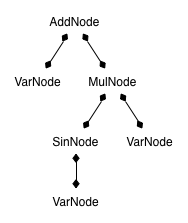
\includegraphics[scale=0.5]{ExpressionTree.png}
    \caption{Illustration de l'expression $(x+x*sin(x))$}
    \label{fig:ExpressionTree}
    \end{center}
\end{figure}
\newpage
\subsection*{Diagramme de classe.}
\begin{figure}[!h]
    \begin{center}
    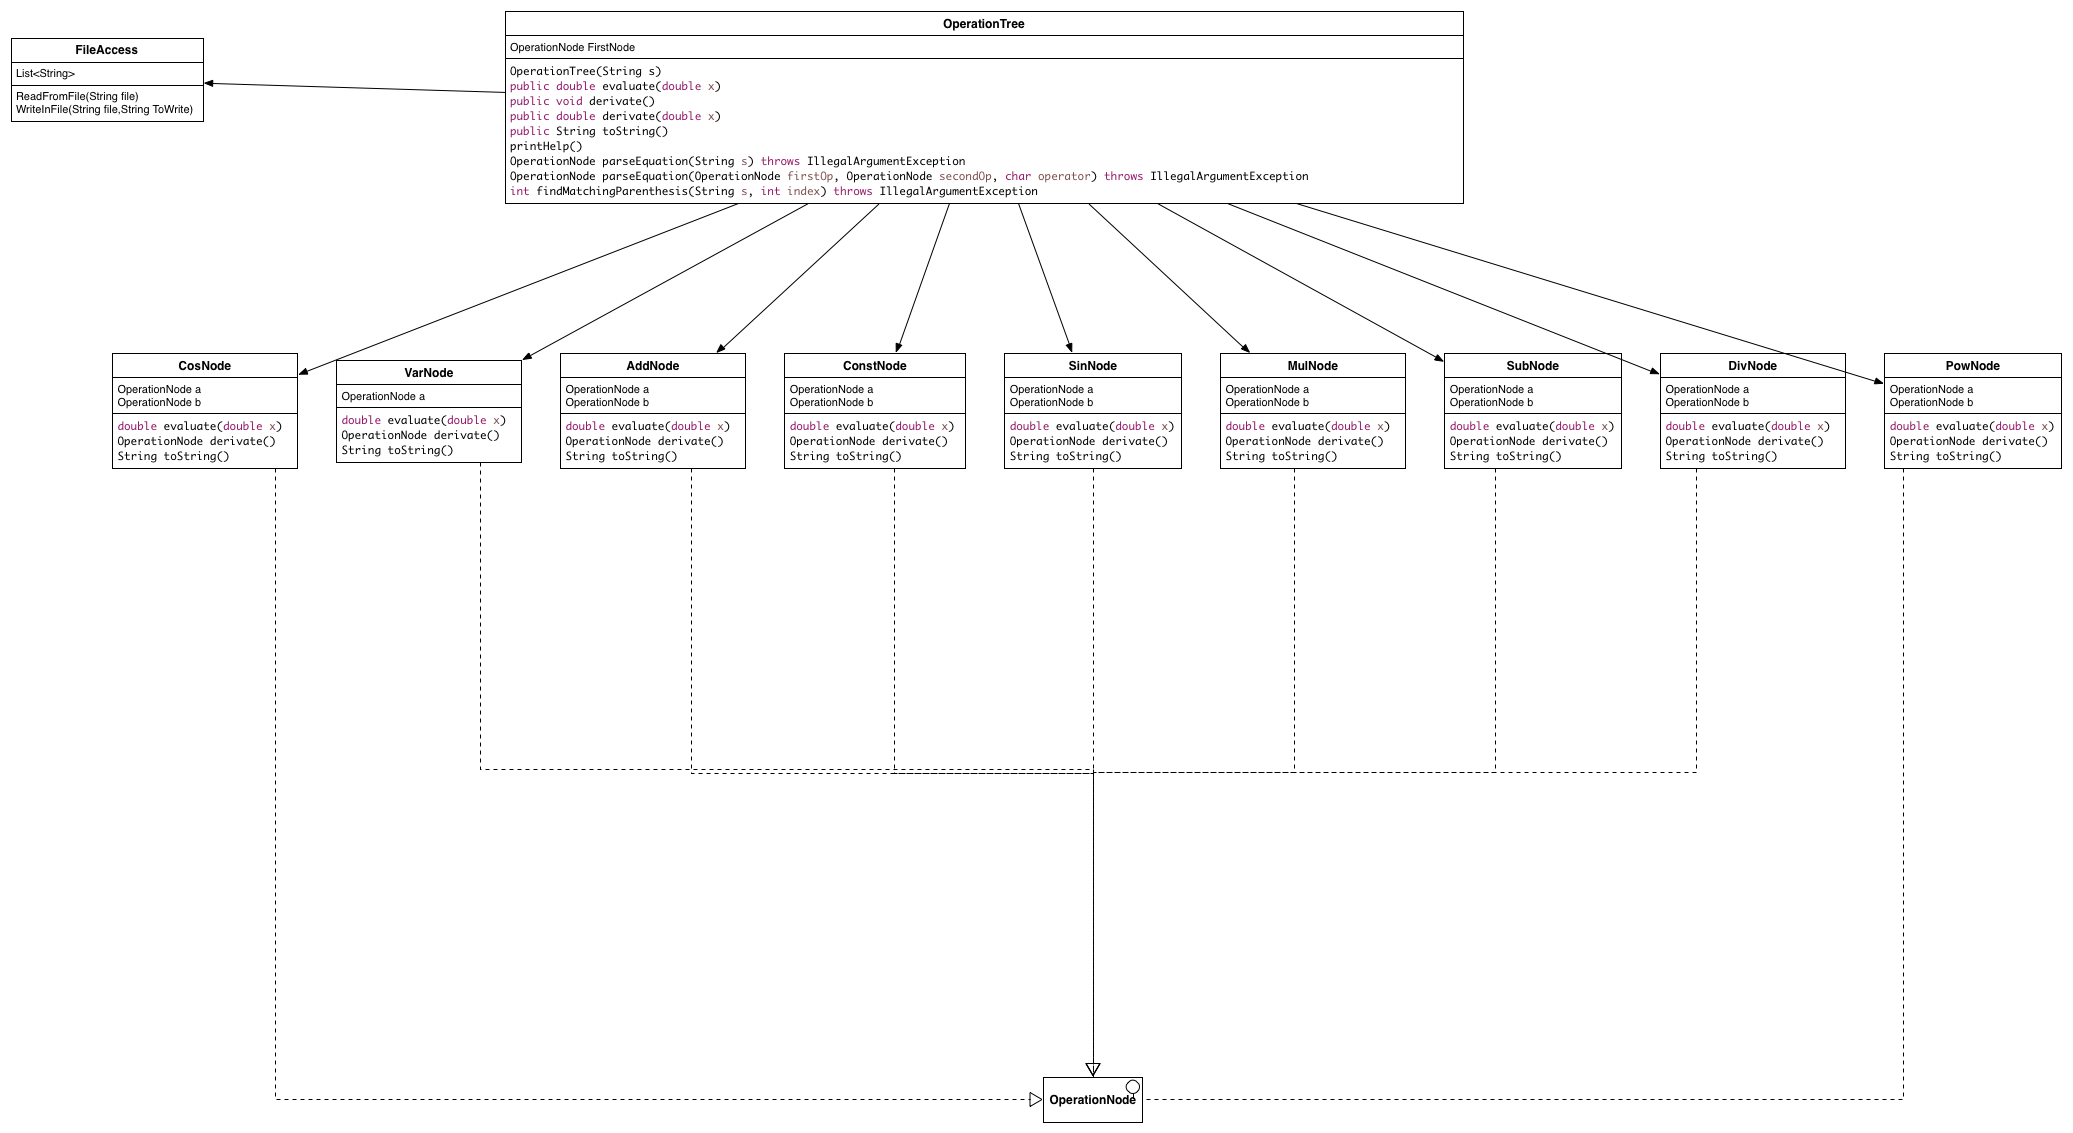
\includegraphics[scale=0.3,angle = 90]{M2_DerivationTree.png}
    \caption{Diagramme de classe de notre programme.}
    \label{fig:ClassDiagram}
    \end{center}
\end{figure}
\section*{Problèmes rencontrés}
\section*{Conclusion}
\end{document}